%DO NOT MESS AROUND WITH THE CODE ON THIS PAGE UNLESS YOU %REALLY KNOW WHAT YOU ARE DOING
\chapter{Study of Classification Algorithms} \label{Study of Classification Algorithms}
We would briefly like to discuss the classification algorithms we have used in our study


\section{ Support Vector Machine (SVM)} \label{ Support Vector Machine (SVM)}
\noindent SVMs are supervised learning algorithms used for classification and regression analysis. A support vector machine constructs a hyperplane or set of hyperplanes in a high or infinite dimensional space, which is then used to separate out and classify the data. Intuitively, a good separation is achieved by the hyperplane that has the largest distance to the nearest training-data point of any class, since in general the larger the margin the lower the generalization error of the classifier. SVM is able to discriminate data that is not linearly separable by using the kernel trick. \par 
\noindent The trick stipulates the original finite-dimensional space to be mapped into a much higher-dimensional space, presumably making the separation easier in that space. This is done by selecting a kernel function to suit the problem. The hyperplanes in the higher-dimensional space are defined as the set of points whose dot product with a vector in that space is constant.

\begin{figure}[H]
\centering
{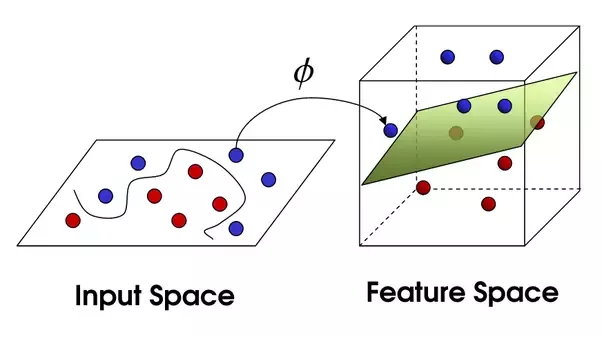
\includegraphics[scale=0.65]{ktr.png}}
\caption{Kernel trick representation}
\end{figure}


\subsection{Pros and Cons associated with SVM} \label{Pros and Cons associated with SVM}

The advantages of SVM are it is effective in high dimensional spaces and in cases where number of dimensions is greater than the number of samples. It uses a subset of training points in the decision function (called support vectors), so it is also memory efficient. It is versatile means different Kernel functions can be specified for the decision function. Common kernels are provided, but it is also possible to specify custom kernels. \par

Despite this it doesn’t perform well when we have large data set because the required training time is higher. It also doesn’t perform very well, when the data set has more noise i.e. target classes are overlapping and SVM doesn’t directly provide probability estimates, these are calculated using an expensive five-fold cross-validation.




\section{Results} \label{Results}
This is the second section of the fourth chapter.
\section{Discussion} \label{Discussion}
This is the third section of the fourth chapter.